\documentclass[10pt, a4paper, spanish]{article}
\usepackage[paper=a4paper, left=1.5cm, right=1.5cm, bottom=1.5cm, top=3.5cm]{geometry}
\usepackage[spanish]{babel}
\selectlanguage{spanish}
\usepackage[utf8]{inputenc}
\usepackage[T1]{fontenc}
\usepackage{indentfirst}
\usepackage{fancyhdr}
\usepackage{latexsym}
\usepackage{lastpage}
\usepackage[colorlinks=true, linkcolor=blue]{hyperref}

\usepackage{listings}
\usepackage{listingsutf8}
\usepackage{color}

\definecolor{codegreen}{rgb}{0,0.6,0}
\definecolor{codegray}{rgb}{0.5,0.5,0.5}
\definecolor{codepurple}{rgb}{0.58,0,0.82}
\definecolor{backcolour}{rgb}{0.95,0.95,0.92}

\lstset{inputencoding=utf8/latin1,
	language=C++,
	basicstyle=\ttfamily,
	keywordstyle=\bfseries\color{blue},
	stringstyle=\color{red}\ttfamily,
	commentstyle=\color{mygreen}\ttfamily,
	morecomment=[l][\color{magenta}]{\#},
	% numbers=left,
	numberstyle=\color{gray},
	backgroundcolor=\color{backcolour},   
	keywordstyle=\color{magenta},
	breakatwhitespace=false,
	breaklines=true,
	captionpos=b,
	keepspaces=true,
	numbersep=5pt,
	showspaces=false,
	showstringspaces=false,
	showtabs=false,
	tabsize=3,
	inputencoding=utf8/latin1
}

% Para que tenga acentos el environment lstlisting
\lstset{
     literate=%
         {á}{{\'a}}1
         {í}{{\'i}}1
         {é}{{\'e}}1
         {ý}{{\'y}}1
         {ú}{{\'u}}1
         {ó}{{\'o}}1
         {ě}{{\v{e}}}1
         {š}{{\v{s}}}1
         {č}{{\v{c}}}1
         {ř}{{\v{r}}}1
         {ž}{{\v{z}}}1
         {ď}{{\v{d}}}1
         {ť}{{\v{t}}}1
         {ň}{{\v{n}}}1                
         {ů}{{\r{u}}}1
         {Á}{{\'A}}1
         {Í}{{\'I}}1
         {É}{{\'E}}1
         {Ý}{{\'Y}}1
         {Ú}{{\'U}}1
         {Ó}{{\'O}}1
         {Ě}{{\v{E}}}1
         {Š}{{\v{S}}}1
         {Č}{{\v{C}}}1
         {Ř}{{\v{R}}}1
         {Ž}{{\v{Z}}}1
         {Ď}{{\v{D}}}1
         {Ť}{{\v{T}}}1
         {Ň}{{\v{N}}}1                
         {Ů}{{\r{U}}}1    
}

\usepackage[Algoritmo]{algorithm}
\usepackage{algpseudocode}
\algrenewcommand\textproc{}% Used to be \textsc Para que el nombre de la función no sea en mayusculas
\usepackage{verbatim}

\usepackage{tabularx} % tablas copadas
% \usepackage{graphicx}
\usepackage{amsmath, amsthm, amssymb}

%\usepackage{makeidx}
\usepackage{paralist} %itemize inline
\usepackage[table]{xcolor}
\usepackage{caratula/caratula}

\usepackage{float}
\usepackage{amsfonts}
\usepackage{sectsty}
\usepackage{charter}
\usepackage{wrapfig}

\usepackage{caption}
%el de arriba funciona si no esta, el de abajo quite el "Figura #" de las imagenes
\captionsetup[figure]{labelformat=empty}

\begin{document}

\titulo{Trabajo práctico II}

\subtitulo{PTHREADS}

\materia{Sistemas Operativos}

\integrante{Cámera, Joel Esteban}{257/14}{joel.e.camera@gmail.com}
\integrante{Lavia, Alejandro Norberto}{43/11}{lavia.alejandro@gmail.com}
\integrante{Guttman, Martín David}{686/14}{mdg\_92@yahoo.com.ar}


\maketitle

\tableofcontents

\newpage
\section{Introducción}

En el presente informe reseñamos las mejoras realizadas al servidor del juego de \textit{HaSObro} para que tener múltiples jugadores a la vez. Para esto, utilizamos la biblioteca \textbf{pthreads} de POSIX para realizar los cambios en el servidor de \textit{backend} así pueda atender a múltiples jugadores.

Como primera parte del mismo, exponemos la implementación de la estructura \textit{Read-Write lock}, donde se utilizan sólo variables de condición de la librería \textbf{pthreads} , y los respectivos test que demuestran que la estructura está libre de inanición y posée el comportamiento esperado. Como segunda parte, presentamos una implementación del servidor de \textit{backend multiusuario} con los detalles implementativos y las decisiónes de diseño del mismo que hacen que permita múltiples clientes jugando simultáneamente.

% \newpage
\section{Implementación \textit{Read-Write Lock}}

Aquí presentamos nuestra implementación del \textit{Read-Write Lock} donde exponemos su estructura y su funcionamiento. En ésta se podría generar el problema de inanición si se presentan los casos en donde haya siempre pedidos de lectura o escritura, al intentar realizar un pedido contrario a estos según el caso éste queda bloqueado. Por ello, también presentamos las medidas tomadas para evitar estos casos.


\subsection{Estructura}

Para poder implementar el \textit{Read-Write Lock} utilizamos una estructura basada en una variable de condición y un mutex, además de dos enteros que cuentan la cantidad de lectores y escritores y un flag.

La estructura es la siguiente:

\begin{itemize}
	\item Mutex: \textbf{m}
	\item Variable de condicion: \textbf{turn}
	\item Contador de lectores: \textbf{reading}
	\item Contador de escritores: \textbf{writers}
	\item Flag: \textbf{writing}
\end{itemize}


\subsection{Función \textit{rlock()}}

\begin{lstlisting}
Pido el mutex

Si la cantidad de escritores es mayor que cero
	Espero el proximo turno

Mientras haya alguien escribiendo
	Esperar el proximo turno

Aumento en uno el contador de la cantidad de lectores

Libero el mutex
\end{lstlisting}

Lo primero realiza esta función es pedir el mutex. Una vez obtenido el mismo, se fija si la cantidad de escritores es mayor que cero y, si lo es, espera al proximo turno. Esto se hace para parar una posible seguidilla de pedidos de lectura que produzcan inanición a los threads que pidan una lectura.

Luego, mientras haya algún thread escribiendo se espera hasta el proximo turno. Esto se hace para garantizar el acceso exclusivo a la sección critica.

Por último, una vez que no haya algún thread escribiendo se aumenta en uno el contador de la cantidad de lectores y se libera el mutex.

\newpage

\subsection{Función \textit{wlock()}}

\begin{lstlisting}
Pido el mutex

Aumento en uno el contador de la cantidad de escritores

Mientras haya alguien escribiendo o la cantidad de lectores es mayor que cero
	Espero el proximo turno

Levanto el flag de escritura

Libero el mutex
\end{lstlisting}

Primero se pide el mutex. Una vez obtenido el mismo se aumenta el contador de la cantidad de escritores en uno.

Luego, mientras haya alguien escribiendo o leyendo, espera al proximo turno. Esto se hace para garantizar el acceso exclusivo a la sección critica ya que si alguien está escribiendo no debería acceder otro para escribir y, también, para que se escriba solamente cuando nadie esté leyendo.

Una vez que no haya nadie escribiendo ni leyendo, se levanta el flag de escritura y se libera el mutex.

~
\subsection{Función \textit{runlock()}}

\begin{lstlisting}
Pedir mutex

Disminuyo en uno el contador de la cantidad de lectores

Si la cantidad de lectores es igual a cero
	Dar turno a todos los que esperan uno

Liberar mutex
\end{lstlisting}

Una vez terminada la lectura, se pide el mutex nuevamente y se disminuye en uno el contador de la cantidad de lectores.

Luego, si ya no hay más lectores se da turno a todos los que esperan uno, tanto lectores como escritores. Y, por último, se libera el mutex.

~
\subsection{Función \textit{wunlock()}}

\begin{lstlisting}
Pido el mutex

Disminuyo en uno el contador de la cantidad de escritores

Bajo el flag de escritura

Doy turno a todos los que esperan uno

Libero el mutex
\end{lstlisting}

Una vez terminada la escritura, se pide el mutex nuevamente, se baja el flag de escritura y se disminuye el contador de la cantidad de escritores.

Luego, se da un turno a todos los que esperan uno, tanto lectores como escritores y se libera el mutex.


~
\subsection{Inanición}

Por lo expuesto anteriormente sobre el funcionamiento de nuestra estructura, ésta contiene los medios suficientes para evitar que una seguidilla de threads con una misma operación hagan que se bloquéen threads con la operación contraria.

En el caso de los lectores, estos esperan a que terminen los escritores de escribir. Y, en el caso de los escritores que no haya threads escriendo o threads leyendo.

~
\subsection{Deadlock}

Para mostrar que en la estructura no se genería deadlock veamos que no se cumplen las condiciones necesarias de Coffman.

\begin{itemize}
	\item \textbf{Exclusión mutua}: Un recurso no puede estar asignado a más de un proceso. 
\newline
	Cómo vimos, todas las operaciones como primera medida realizan un lock con el mutex, esto garantiza que el acceso a un recurso le pertenece a un sólo thread y todos los que quieran utilizarlo esperan hasta que el que lo está utilizando realice un unlock. Si se cae en una variable de condición se liberan los mutex pero todos los threads caerían también en la misma variable de condición y éstas están dentro de ciclos donde, si se quere escribir se espera a que terminen de escribir y que hayan leído los lectores, o si se quiere leer que terminen de escribir. Entonces los lectores son los únicos que podrían entrar varios a la vez pero no modificarían las variables, en cambio los que quieren escribir tienen acceso exclusivo.

	\item \textbf{Hold and wait}: Los procesos que ya tienen algún recurso pueden solicitar otro.
\newline
	En este caso, esto ocurriría si un thread no puede leer o escribir se quede con el mutex hasta que pueda realizar la operación. Pero esto no sucede ya que los mutex se liberan en el momento que el thread llama a la función \textbf{pthread\_cond\_wait()} para esperar que la condición se cumpla para realizar la operación.
	
	\item \textbf{No Preemption}: Un recurso puede ser liberado solamente de forma voluntaria por el proceso que lo retiene.
\newline
	En este caso, no podría suceder esto ya que los threads que quieran acceder a un recurso que esta siendo utilizado deben esperar a que la variable de condición sea verdadera y ésta sólo puede ser liberada por el proceso que tiene el recurso.
	
	\item \textbf{Espera circular}: Tiene que haber un ciclo de $N \geq 2$, tal que $P_i$ espera un recurso que tiene $P_{i+1}$.
\newline
	Cómo el recurso al que se quiere acceder es único en este caso, no puede haber espera circular.
\end{itemize}


\subsection{Tests}

Para probar nuestra implementación de \textit{Read-Write Lock} realizamos tres tipos de test que se pueden encontrar en la carpeta \textbf{locks} junto con la implementación de la estructura. En cada uno de estos lanzamos 10.000 threads.

Pasamos a explicar sobre ellos:

\begin{enumerate}
	\item En este primer test creamos 5000 threads escritores y 5000 threads lectores todos con un único número, siendo los pares los threads lectores y los impares los escritores. Lo que se hace es guardar en un arreglo cuantos lectores hubo hasta el momento de que esta un thread escritor y viceversa.
	\newline
	Una vez que corrieron todos los threads, se revisa ese arreglo y se mira si la cantidad de threads lectores o escritores está dentro de un rango de 15 threads (tomado este número de forma arbitraria) de diferencia según el thread del índice. Si está por debajo de ese rango quiere decir que se tarda en leer (si el índice es par) o en escribir (si el índice es impar). Si está por arriba del rango quiere decir que tiene una prioridad mayor leer (si el índice es par) o escribir (si el índice es impar).

	\item En el segundo test realizamos un experimento con la misma logica que el primero pero con la diferencia que un 90\% de los threads son escritores y un 10\% threads son lectores.

	\item En este tercer y último test tambíen realizamos un experimento con la misma logica que el primero pero esta vez un 90\% de los threads son lectores y un 10\% son escritores.
\end{enumerate}
\newpage
\section{Servidor de backend}

En esta sección vamos a detallar los cambios realizados al servidor de backend. Originalmente contábamos con una implementación mono cliente y nuestra tarea es adaptar esta implementación para permitir múltiples clientes en simultaneo bien sincronizados.

\subsection{Backend mono cliente}

Inicialmente se setean los tableros del juego de $n$ por $m$ y también el socket de tipo \textbf{INET} con protocolo \textbf{TCP}. Una vez hecho esto, se queda a la espera de una conexión entrante y, cuando llega, la acepta y establece el socket entre el cliente y el servidor. Luego, se cierra el socket del servidor para nuevas conexiones. El flujo de ejecución se queda atendiendo las jugadas del cliente, hasta que este finalice. El problema de ésta implementación es que no solo se cierra el socket del servidor sino que, además, si no se hubiera hecho, el servidor se queda ejecutando la rutina de atención del único cliente siendo imposible aceptar nuevas conexiones.

\begin{figure}[H]
  \begin{center}
	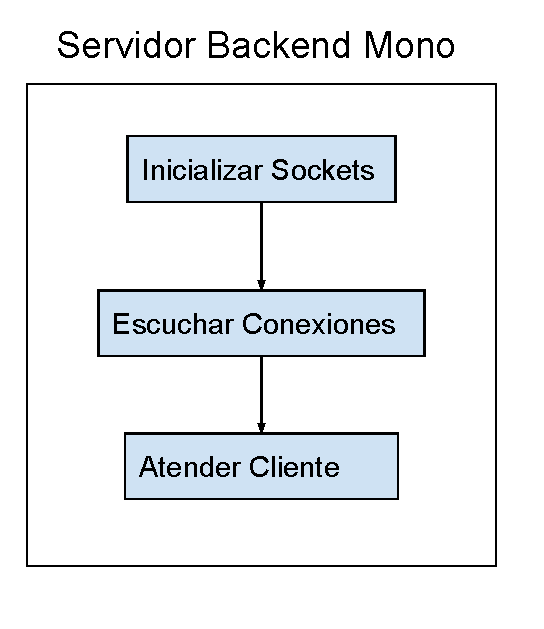
\includegraphics[scale = 0.5]{./imagenes/so_tp2_1.pdf}
	\caption{Diagrama el funcionamiento del backend mono.}
	\label{fig:fig1}
  \end{center}
\end{figure}

\subsection{Backend múltiples clientes}

El cambio más importante para darle soporte multiusuario al backend radica en el uso de threads de la librería \textbf{pthreads}. Inicialmente realizamos las mismas operaciones que el backend mono para setear el tablero y los sockets y luego nos quedamos a la espera de conexiones entrantes. Pero, al momento de recibir una nueva conexión en lugar de derivar todo el flujo de ejecución del programa a la rutina de atención del cliente, creamos un nuevo hilo de ejecución (\textit{thread}) que se encargara de ello con la función \textbf{pthread\_create}. También, mantenemos abierto el socket a la espera de nuevos clientes y tenemos ejecutándose concurrentemente la rutina que acepta a los clientes y las rutinas que atienden a los cliente así puedan conectarse muchos clientes en el juego.

\begin{figure}[H]
  \begin{center}
	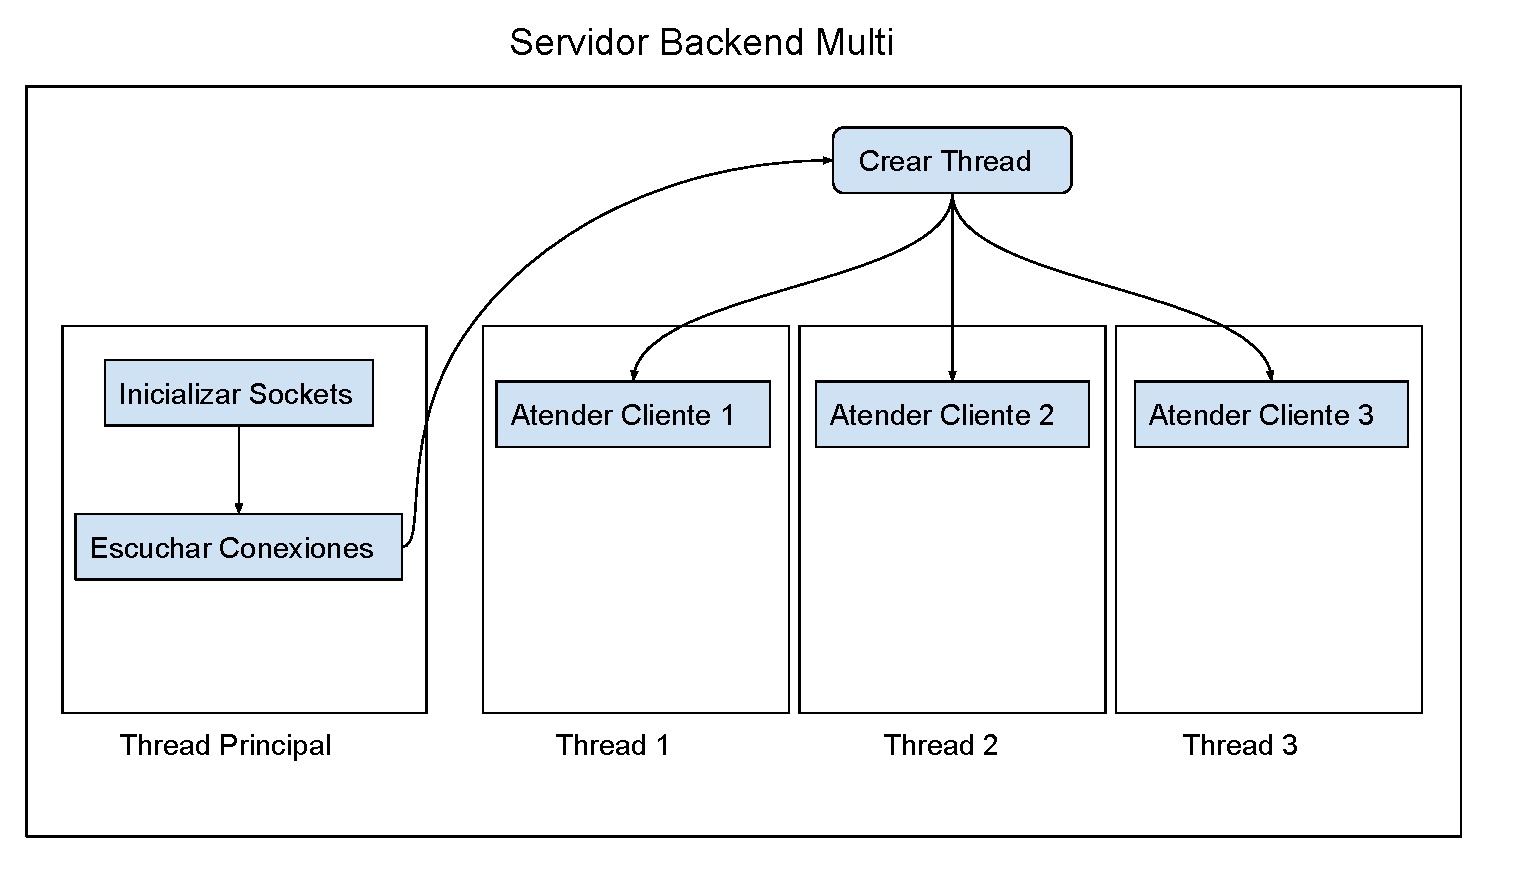
\includegraphics[scale = 0.4]{./imagenes/so_tp2_2.pdf}
	\caption{Diagrama ilustrativo del backend multiusuario}
	\label{fig:fig2}
  \end{center}
\end{figure}

La siguiente cuestión a resolver para mantener la correcta sincronización entre los hilos y estar libres de condiciones de carrera, fue determinar las zonas críticas del servidor. El servidor cuenta con dos variables globales compartidas por todos los threads, estas son \textit{tablero\_temporal} y \textit{tablero\_confirmado}. Estas variables son leídas y escritas con las distintas acciones de los clientes, por lo tanto estas serán nuestras secciones críticas a las cuales debemos garantizar el acceso exclusivo para mantener la coherencia. Esto lo hacemos aprovechando los mecanismos provistos por la clase implementada anteriormente \textbf{RWLock}, así que agregamos dos instancias globales de esta clase, \textit{lock\_tablero\_temporal} y \textit{lock\_tablero\_confirmado} con el fin de garantizar el acceso exclusivo a las secciones críticas. Vamos a listar las funciones del juego con los cambios efectuados:

\begin{itemize}
	\item Atender jugador:
		\begin{itemize}
			\item Colocar una carta: En esta operación estamos modificando el tablero temporal con la carta colocada, solicitamos el \textit{write-lock} del tablero temporal, efectuamos el cambio, y luego lo liberamos \textit{write-unlock}.
			\item Confirmar jugada: Necesitamos escribir en el tablero confirmado la jugada del cliente pedimos \textit{write-lock} en el tablero confirmado por cada escritura realizada de la jugada y al finalizar liberamos \textit{write-unlock}.
		\end{itemize}
	\item Enviar tablero: Enviamos el tablero confirmado a un cliente y para eso leemos el tablero confirmado, así que solicitamos el \textit{read-lock}, efecutamos la lectura y luego hacemos un \textit{read-unlock} 
	\item Quitar cartas: El tablero temporal debe ser limpiado, se debe escribir en todas sus coordenadas, por ello realizamos un \textit{write-lock}, limpiamos la coordenada y luego un \textit{write-unlock}.
	\item Es ficha valida: En esta operación comprobamos si una jugada es válida, para ello debemos leer tanto el tablero temporal como el tablero confirmado, solicitamos con sus respectivas instancias de \textbf{RWLock} el \textit{read-lock} cada vez que el casillero necesite ser leído, luego lo liberamos con \textit{read-unlock}
\end{itemize}

Finalmente, luego de garantizar el acceso exclusivo a las secciones críticas, sólo nos queda finalizar el thread cuando el cliente términe su conexión con el servidor, para ello agregamos en la rutina encargada de terminar el cliente un llamado a \textbf{pthread\_exit} que indica que el hilo actual ha finalizado.


% \newpage

\end{document}
